
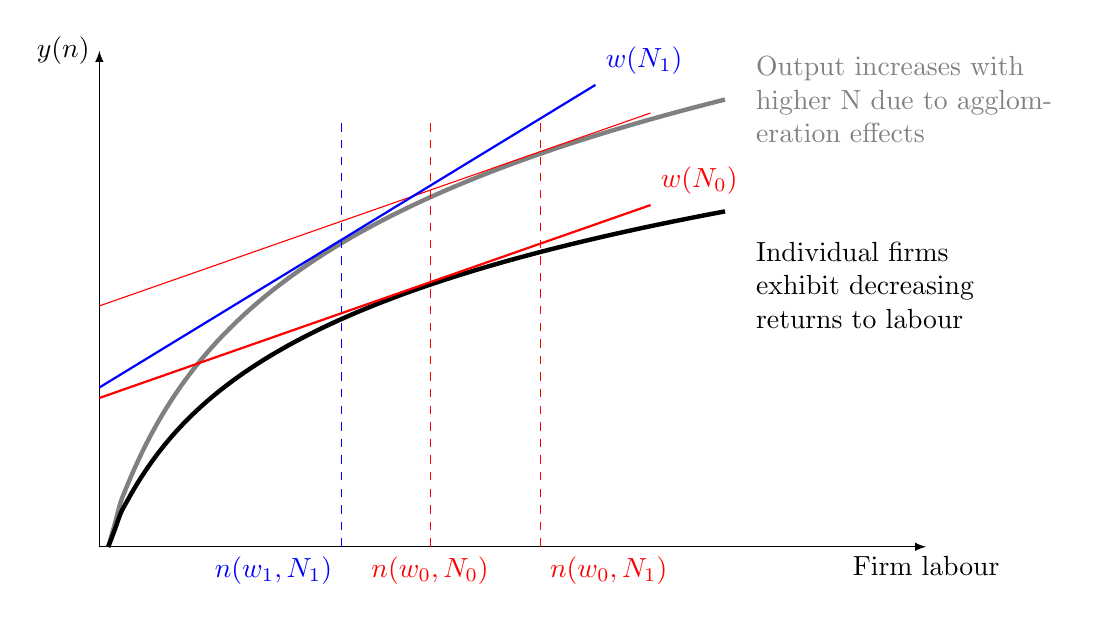
\begin{tikzpicture}[scale=.7, my plot/.style={thick, smooth, samples=100, domain=0.1:1.5},
plot2/.style={thick, smooth, samples=100, domain=0.1:9},
                    my grid/.style={dashed,opacity=0.5, every node/.style={black,opacity=1}},
                    my axis/.style={latex-latex}]
 
 \draw[my axis] (0,9)node[left] {$y(n)$} --(0,0)-- (15, 0) node[below] {Firm labour}; %creates the axis a little 

\coordinate (origin) at (0,0);
\def\x{0.45}
\def\y{2.1}
\def\b {$15/(2*ln(\y)+.05)$};
\coordinate (Uy) at (\y,{2*ln(\y)+.05});


\begin{scope}[ yscale=6, xscale=8]% shift={(1.9,0)} ,
	\coordinate (Uy) at (\y, {2.3+ln(\y)});
  \draw[my plot, ultra thick, gray] (0,0) plot ({\x-.08},{1.15+ln(\x)/2})node[right=.25cm, text width=3.9cm]{Output\ increases\ with\ higher\  N\ due\ to\ agglomeration\  effects}; % production function for generic ferm
\draw[dashed, red](.75, 0)node[below]{$n(w_0, N_0)$} --(.75, 1.3);
\draw[dashed, thin, red](1., 0)node[below right]{$n(w_0, N_1)$} --(1.0, 1.3);
\draw[dashed, blue](.55, 0)node[below left]{$n(w_1, N_1)$} --(.55, 1.3);
\end{scope}

\begin{scope}[ yscale=4.5, xscale=8]% shift={(1.9,0)} ,
	\coordinate (Uy) at (\y, {2.3+ln(\y)});
  \draw[my plot, ultra thick] (0,0) plot ({\x-.08},{1.15+ln(\x)/2})node[below right=.25cm, text width=3.9cm]{Individual firms\\ exhibit decreasing\\ returns to labour}; % production function for generic ferm
\end{scope}

 \draw [thin, red, thick ](0,2.7)--(10, 6.2)node[above right]{$w(N_0)$};   %wage line
  \draw [thin, red ](0,4.37)--(10, 7.87);%node[below right]{$w(N_0)$}; 
  \draw [thick, blue](0,2.89)--(9, 8.38)node[above right]{$w(N_1)$};   %wage line

\end{tikzpicture}
